\documentclass[xcolor=pdftex,dvipsnames]{beamer}
\usetheme{Frankfurt}
\setbeamertemplate{headline}{}


\usepackage{graphicx}
\usepackage{amsmath}
\usepackage{fancybox,multirow}

% VISEO Style ------------------------
% Colors
\definecolor{viseoblue}{RGB}{0,51,102}
\setbeamercolor{titlelike}{fg=White,bg=viseoblue}
\setbeamercolor{frametitle}{fg=White,bg=viseoblue}
 
\newcommand{\btVFill}{\vskip0pt plus 1filll}

% VISEO Logo on every slide
\titlegraphic{\vfill 
\includegraphics[height=1cm]{./fig/logo_viseo_big.png}}
% \setbeamertemplate{footline}{\hspace{0.1cm}{\color{viseoblue} {\tiny \texttt{parantapa.goswami@viseo.com}}} \hfill 
\includegraphics[height=0.5cm]{./fig/logo_viseo.png}\hspace{0.1cm}~}
\setbeamercolor{footlinecolor}{fg=white,bg=viseoblue}
\setbeamertemplate{footline}{
  \begin{beamercolorbox}[wd=\paperwidth,ht=1ex,dp=1ex,right]{}
    \hfill 
\includegraphics[height=0.32cm]{./fig/logo_viseo_small.png}~
  \end{beamercolorbox}
  \begin{beamercolorbox}[wd=\paperwidth,ht=2.25ex,dp=1ex,center]{footlinecolor}%
    \usebeamerfont{title in head/foot}\textbf{\inserttitle}
  \end{beamercolorbox}
  % \begin{beamercolorbox}[wd=.33\paperwidth,ht=2.25ex,dp=1ex,right]{footlinecolor}%
  %   \usebeamerfont{date in head/foot}\insertshortdate{}
  % \end{beamercolorbox}
}

% To remove the navigation symbols from the bottom of all slides uncomment this line
\setbeamertemplate{navigation symbols}{}

\title{Supervised Learning: Regression}
\author[Parantapa]{Parantapa Goswami}
\institute[Viseo]{\color{viseoblue} Viseo R\&D\\Grenoble, France\\{\tiny \texttt{parantapa.goswami@viseo.com}}}


\begin{document}
\frame[plain]{
\titlepage
}

%---------------------
\begin{frame}
  \frametitle{Classification}
  \framesubtitle{IRIS Classification, Ronald Fisher (1936)}
  \begin{minipage}{0.69\linewidth}
    \begin{center}
      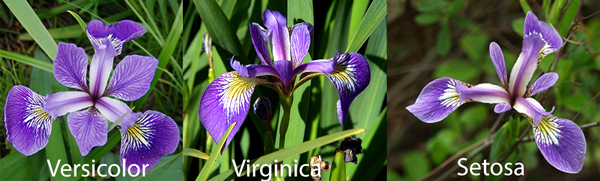
\includegraphics[scale=0.3]{./fig/iris_classes.png}\\ \vspace{0.2cm}
      \pause
      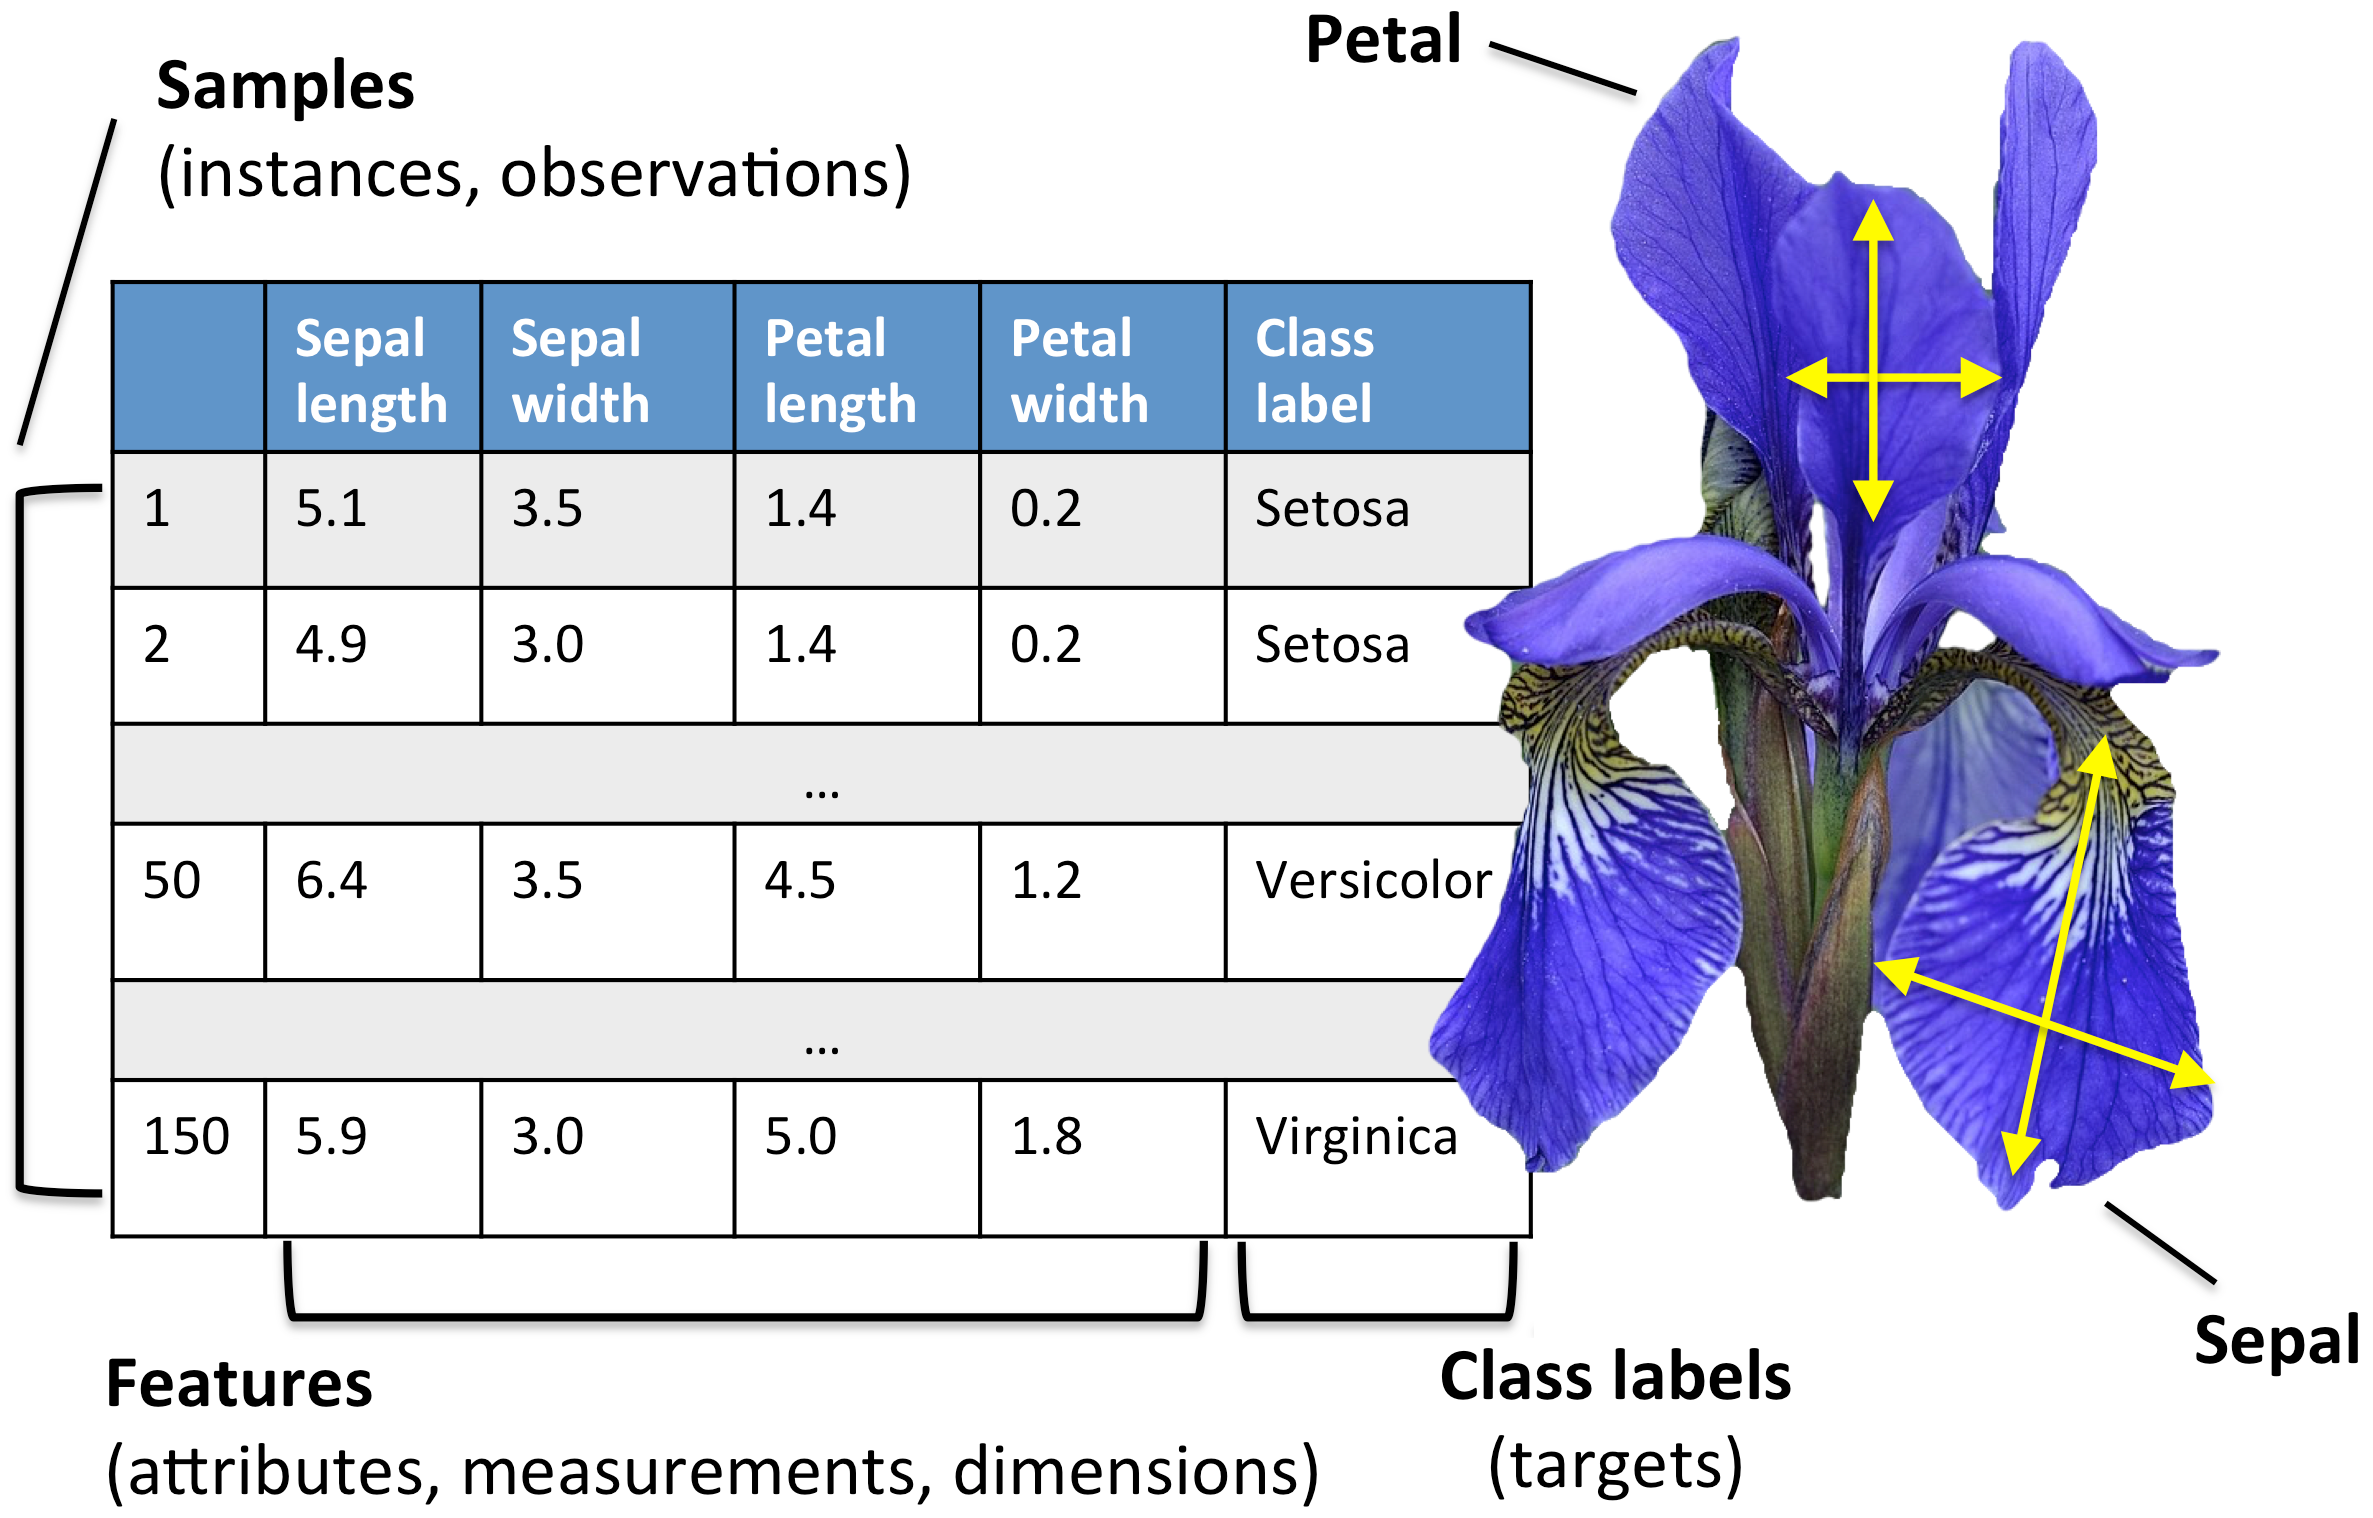
\includegraphics[scale=0.1]{./fig/iris_features.png}
    \end{center}
  \end{minipage}
  \begin{minipage}{0.29\linewidth}
    \begin{itemize}
    \pause
    \item discrete valued output
    \pause
    \item what if output is continuous?
    \end{itemize}
  \end{minipage}
\end{frame}

%---------------------
\begin{frame}
  \frametitle{Regression}
  \vspace{-0.2cm}
  \begin{center}
    \only<1>{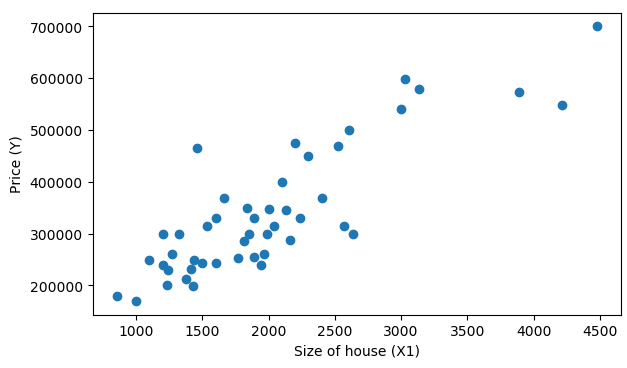
\includegraphics[scale=0.5]{./fig/house_price_area.png}}
    \only<2->{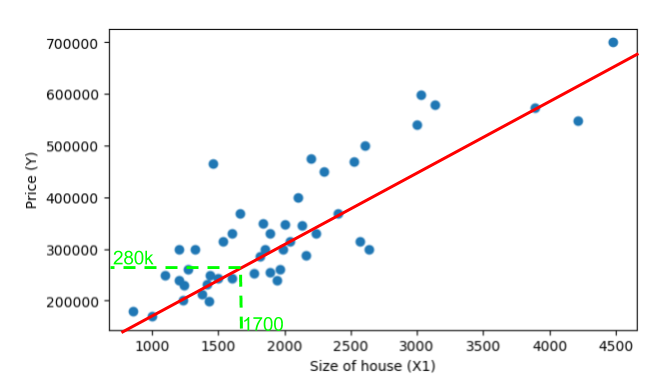
\includegraphics[scale=0.35]{./fig/house_price_area_2.png}}
  \end{center}
  \pause \pause
  \begin{minipage}{0.47\linewidth}
    \begin{block}{}
      \underline{Supervised Learning}\\ \vspace{0.2cm}
      \alert{Right answers} are given
     \end{block}
   \end{minipage}\hfill
  \pause
  \begin{minipage}{0.47\linewidth}
    \begin{block}{}
      \underline{Regression Problem}\\ \vspace{0.2cm}
      Predict \alert{real valued} output
    \end{block}
  \end{minipage}
\end{frame}

%---------------------
\begin{frame}
  \frametitle{Training Set}
  \begin{minipage}{0.47\linewidth}
    \begin{tabular}[h]{c | c}
      Size of house   & Price in \\
      in feet$^2$ (x) & 1000\$s (y) \\\hline
      2104 & 460 \\
      1416 & 232 \\
      1534 & 315 \\
      $\vdots$ & $\vdots$
    \end{tabular}
    \begin{block}{}
      \alert{$m$} $\rightarrow$ number of examples\\
      \alert{$x$} $\rightarrow$ input variable/features\\
      \alert{$y$} $\rightarrow$ output variable/target\\
      \alert{$(x^i, y^i)$} $\rightarrow$ $i^{th}$ training example
    \end{block}
  \end{minipage} \hfill
  \pause
  \begin{minipage}{0.47\linewidth}
    \begin{center}
      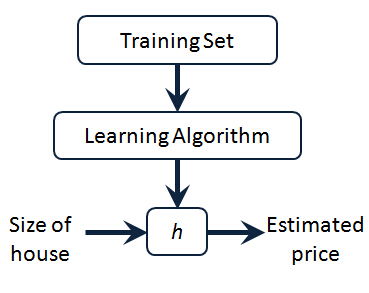
\includegraphics[scale=0.55]{./fig/training_schema.png}\\ 
      Hypothesis \alert{$h: x \rightarrow y$}
    \end{center}
    \pause
    \begin{block}{}
      \begin{center}
        $y = h_{\theta}(x) = \theta_0 + \theta_1 x$
        \pause
        \alert{Univariate Linear Regression}
      \end{center}
    \end{block}
  \end{minipage}
\end{frame}

%---------------------
\begin{frame}
  \frametitle{How to choose the parameters?}
  \begin{block}{}
    \begin{center}
      $y = h_{\theta}(x) = \theta_0 + \theta_1 x$
    \end{center}
  \end{block}
  \pause
  \begin{itemize}
  \item Different $\theta_0$ and $\theta_1$ will generate different lines
    \begin{center}
      \only<2>{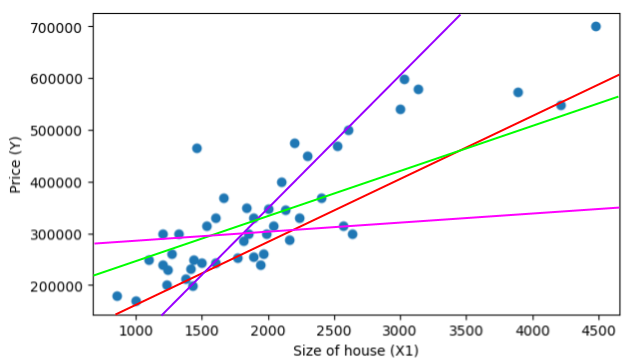
\includegraphics[scale=0.32]{./fig/house_price_linefit.png}}
      \only<3->{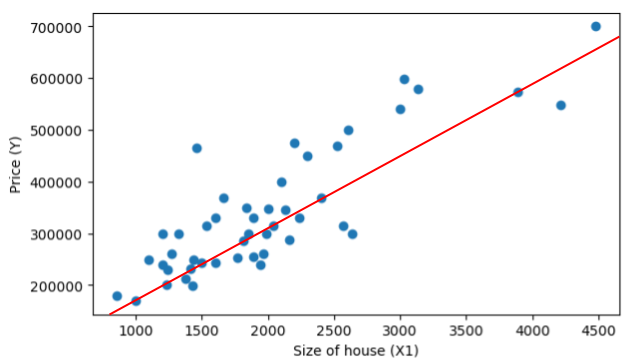
\includegraphics[scale=0.32]{./fig/house_price_linefit_2.png}}
    \end{center}
  \pause \item Need to choose \alert{best} $\theta_0$ and $\theta_1$ 
  \end{itemize}
  \pause
  \begin{block}{}
    Idea: Choose $\theta_0$ and $\theta_1$ so that $h_{\theta}(x)$ is close to given outputs $y$ in the training examples $(x,y)$  
  \end{block}
\end{frame}

%---------------------
\begin{frame}
  \frametitle{Defining a Cost}
  \begin{block}{}
    \begin{center}
      $y = h_{\theta}(x) = \theta_0 + \theta_1 x$
    \end{center}
  \end{block}
  \begin{block}{}
    Idea: Choose $\theta_0$ and $\theta_1$ so that $h_{\theta}(x)$ is close to given outputs $y$ in the training examples $(x,y)$  
  \end{block}
  \pause
  \begin{block}{Cost Function: Mean Squared Error}
    \only<2>{\[ min_{\theta_0, \theta_1} \;\; (h_{\theta}(x) - y)^2 \]}
    \only<3>{\[ min_{\theta_0, \theta_1}\;\; \frac{1}{2m} \sum_{i=1}^m (h_{\theta}(x^i) - y^i)^2 \]}
    \only<4->{\[J(\theta_0, \theta_1) = \frac{1}{2m} \sum_{i=1}^m (h_{\theta}(x^i) - y^i)^2 \]\[ min_{\theta_0, \theta_1} \; J(\theta_0, \theta_1)\]}
  \end{block}
  \pause \pause \pause
  \begin{minipage}{0.47\linewidth}
    \begin{block}{}
      For fixed $\theta_0$ and $\theta_1$, $h_{\theta}$ is a function of $x$
     \end{block}
   \end{minipage}\hfill
  \pause
  \begin{minipage}{0.47\linewidth}
    \begin{block}{}
      $J(\theta_0, \theta_1)$ is a function of the parameters $\theta_0$ and $\theta_1$
    \end{block}
  \end{minipage}
\end{frame}
  
%---------------------
\begin{frame}
  \frametitle{More about the Cost}
  \pause
  \begin{minipage}{0.47\linewidth}
    For fixed $\theta_0$ and $\theta_1$, $h_{\theta}$ is a function of $x$
    \begin{center}
      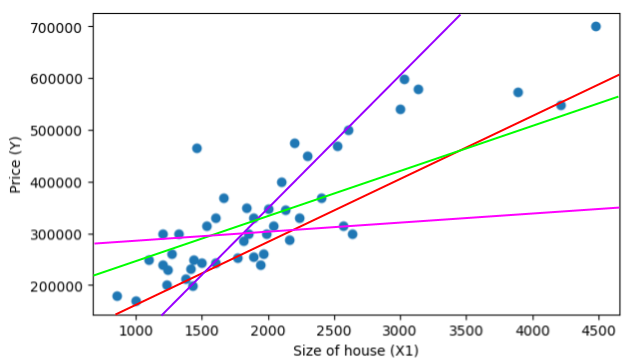
\includegraphics[scale=0.25]{./fig/house_price_linefit.png}
    \end{center}
   \end{minipage}\hfill
  \pause
  \begin{minipage}{0.47\linewidth}
    $J(\theta_0, \theta_1)$ is a function of the parameters $\theta_0$ and $\theta_1$
    \begin{center}
      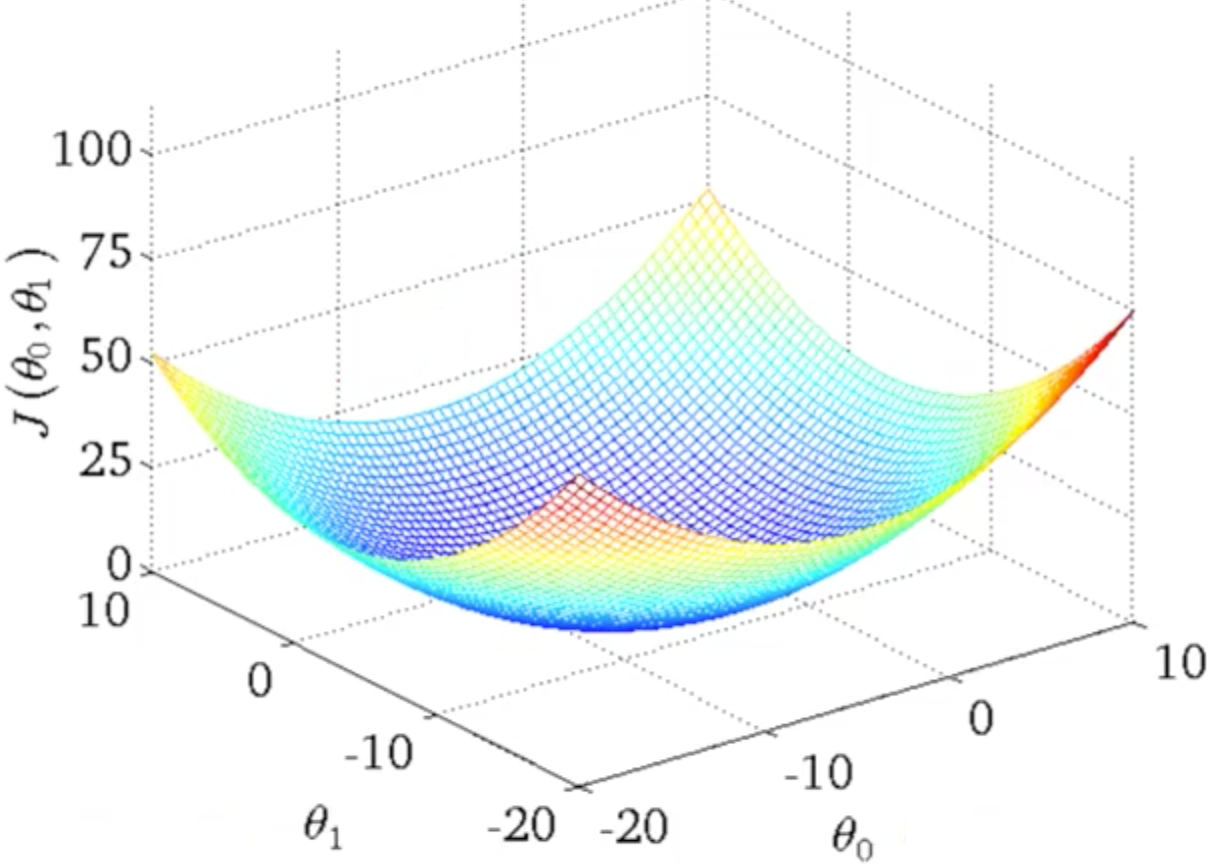
\includegraphics[scale=0.25]{./fig/plot_j_theta.png}
    \end{center}
  \end{minipage}
  \pause
  \begin{itemize}
  \item Goal: to find a $\hat{\theta}_0$ and $\hat{\theta}_1$ providing minimum $J(\theta_0, \theta_1)$
  \item Corresponding hypothesis will be the trained model: $h_{\hat{\theta}}(x) = \hat{\theta}_0 + \hat{\theta}_1x$
  \item $J(\theta_0, \theta_1)$ is convex: can be minimized using \alert{Gradient Descent}
  \end{itemize}
\end{frame}

%---------------------
\begin{frame}
  \frametitle{Multiple Features}
  \begin{center}
    \only<1>{
    \begin{tabular}[h]{c | c}
      Size of house   & Price in \\
      in feet$^2$ (x) & 1000\$s (y) \\\hline
      2104 & 460 \\
      1416 & 232 \\
      1534 & 315 \\
      $\vdots$ & $\vdots$
    \end{tabular}}
    \only<2->{
    \begin{tabular}[h]{c | c | c | c}
      Size of house   & Number of & Number of & Price in \\
      in feet$^2$ (x) & bedrooms  & Floors    & 1000\$s (y) \\\hline
      2104 & 5 & 1 & 460 \\
      1416 & 3 & 2 & 232 \\
      1534 & 3 & 2 & 315 \\
      $\vdots$ & $\vdots$ & $\vdots$ & $\vdots$
    \end{tabular}}
  \end{center}
  \pause
  \begin{block}{}
    \alert{$n$} $\rightarrow$ number of features\\
    \alert{$\vec{x^i}$}$\rightarrow$ $i^{th}$ input is now a $n$-dimensional vector\\
    \alert{$x^i_j$}$\rightarrow$ $j^{th}$ feature of the $i^{th}$ input
  \end{block}
  
\end{frame}

%---------------------
\begin{frame}
  \frametitle{Multivariate Linear Regression}
  \begin{block}{Hypothesis}
    \begin{center}
      $y = h_{\vec{\theta}}(x) = \theta_0 + \theta_1 x_1 + \theta_2 x_2 + \ldots + \theta_n x_n$
    \end{center}
  \end{block}
  \pause
  \begin{block}{Cost Function}
    \begin{center}
      $J(\theta_0, \theta_1, \theta_2, \ldots, \theta_n) = \frac{1}{2m} \sum_{i=1}^m (h_{\vec{\theta}}(\vec{x^i}) - y^i)^2$
    \end{center}
  \end{block}
  \pause
  \begin{itemize}
  \item Goal: to find $\hat{\theta}_0, \ldots, \hat{\theta}_n$ providing minimum $J(\theta_0, \ldots, \theta_n)$
  \item Here also, $J(\theta_0, \ldots, \theta_n)$ is convex: thus can be minimized using \alert{Gradient Descent}
  \end{itemize}
\end{frame}

% ---------------------
\begin{frame}
  \frametitle{Time Series}
  \begin{block}{}
    A time series is a sequence of observations $s_t \in \mathbb{R}$, usually ordered in time.
  \end{block}

  Examples of time series can be found in every scientific and applied domain:
  \begin{itemize}
  \item Meteorology: weather variables, like temperature, pressure, wind.
  \item Economy and finance: economic factors (GNP), financial indexes, exchange rate, spread.
  \item Marketing: activity of business, sales.
  \item Industry: electric load, power consumption, voltage, sensors.
  \item Bio-medicine: physiological signals (EEG), heart-rate, patient temperature.
  \item Web: clicks, logs.
  \end{itemize}
\end{frame}

% ---------------------
\begin{frame}
  \frametitle{Time Series Forecasting}
  \begin{block}{}
    Time series forecasting is the use of a model to predict future values of a time series based on previously observed values.
  \end{block}

  \pause
  To do that:
  \begin{enumerate}
  \item Understand or model the stochastic mechanisms generating the data
  \item This model is used to forecast the future values based on the history
  \end{enumerate}
  \pause
  Examples:
  \begin{itemize}
  \item Weather forecasting.
  \item Sales prediction.
  \item Stock market forecasting.
  \end{itemize}
\end{frame}

% ---------------------
\begin{frame}
  \frametitle{Formalizing Time Series Forecasting}
  \begin{itemize}
  \item Assume we have a time series: \[ x_1, x_2, \ldots, x_N\]
    \pause
  \item $T$ observed values: also known as \alert{history size}
    \pause
  \item Need to forecast $T'$ future values: also known as \alert{forecast horizon}
    \pause
  \item We want to model the relation: \[ (x_{T+1}, x_{T+2}, \ldots, x_{T+T'}) = r(x_1, x_2, \ldots, x_T)\]
  \end{itemize}
\end{frame}

% ---------------------
\begin{frame}
  \frametitle{Constructing Regression Matrix}
  \begin{itemize}
  \item To learn a regression model: multiple examples of feature value pairs are required
    \pause
  \item Moving window method:
    \only<2>{\[ x_1, x_2, \ldots, x_T, x_{T+1}, x_{T+2}, \ldots x_{T+T'}, x_{T+T'+1}, \ldots \]}
    \only<3>{
      \[ \underbrace{x_1, x_2, \ldots, x_T}_{\text{history}}, \underbrace{x_{T+1}, x_{T+2}, \ldots, x_{T+T'}}_{\text{horizon}}, x_{T+T'+1}, \ldots \]
      \[
      X = 
        \begin{bmatrix}
          x_1 & x_2 & \dots & x_T \\
        \end{bmatrix}
        \quad
        Y =
        \begin{bmatrix}
          x_{T+1} & x_{T+2} & \dots & x_{T+T'} \\
        \end{bmatrix}
      \]
    }
    \only<4>{
      \[ x_1, \underbrace{x_2, x_3, \ldots, x_T, x_{T+1}}_{\text{history}}, \underbrace{x_{T+2}, x_{T+3}, \ldots, x_{T+T'+1}}_{\text{horizon}}, x_{T+T'+2}, \ldots \]
      \[
      X = 
        \begin{bmatrix}
          x_1 & x_2 & \dots & x_T \\
          x_2 & x_3 & \dots & x_{T+1} \\
        \end{bmatrix}
        \quad
        Y =
        \begin{bmatrix}
          x_{T+1} & x_{T+2} & \dots & x_{T+T'} \\
          x_{T+2} & x_{T+3} & \dots & x_{T+T'+1} \\
        \end{bmatrix}
      \]
    }
    \only<5->{
      \[ x_1, x_2, \underbrace{x_3, \ldots, x_{T+1}, x_{T+2}}_{\text{history}}, \underbrace{x_{T+3}, x_{T+4}, \ldots, x_{T+T'+2}}_{\text{horizon}}, x_{T+T'+3}, \ldots \]
      \[
      X = 
        \begin{bmatrix}
          x_1 & x_2 & \dots & x_T \\
          x_2 & x_3 & \dots & x_{T+1} \\
          x_3 & x_4 & \dots & x_{T+2} \\
        \end{bmatrix}
        \quad
        Y =
        \begin{bmatrix}
          x_{T+1} & x_{T+2} & \dots & x_{T+T'} \\
          x_{T+2} & x_{T+3} & \dots & x_{T+T'+1} \\
          x_{T+3} & x_{T+4} & \dots & x_{T+T'+2} \\
        \end{bmatrix}
      \]
    }
    \pause \pause \pause \pause
    \item Regression models are learned on input $X$ and output $y$
  \end{itemize}
\end{frame}

% ---------------------
\begin{frame}
  \frametitle{A Good ML Course}
    \begin{itemize}
    \item Introduction to Machine Learning. Course by  Andrew Ng. (Youtube)
    \end{itemize}
\end{frame}

% ---------------------
\begin{frame}
  \begin{center}
    \Large Hands On! \\ \vspace{0.3cm}
    
\includegraphics[scale=0.3]{./fig/hands_on.png}
  \end{center}
  \begin{itemize}
  \item \texttt{1\_MachineLearning\_Regression}
  \item \texttt{2\_TimeSeriesForecasting}
  \end{itemize}
\end{frame}

\end{document}
